\chapter{Fundamentação Teórica}
\label{cap:fundamentacao}
Neste capítulo será abordado sobre os principais conceitos e tecnologias utilizadas no desenvolvimento deste projeto, do hardware à aplicação móvel, iniciando pelo conceito principal, a Internet das Coisas.

% ---
\section{Internet das Coisas}
\label{fund:iot}
Com o intuito de ampliar a internet atual, interligando os objetos do nosso cotidiano, animais e humanos em uma única rede, foi criado a Internet das Coisas, IoT, também conhecida como internet de todas as coisas. Para tal, os objetos viram objetos inteligentes, possuindo capacidade de comunicação associados com sensores que fornecem dados para outros dispositivos. Estes objetos, conectados a IoT, se comunicam via internet, trocando dados em tempo real, transmitindo informações acerca do ambiente que estão inseridos e/ou até mesmo dos seus respectivos estados. 

Deste modo, é adicionando uma nova gama de possibilidades, trazendo grandes benefícios para ambientes domésticos, mas principalmente para a zona industrial. No primeiro caso, aplicações, tais como: aprendizagem reforçada, monitoramento e vigilância inteligentes e vida assistida têm despontado entre aquelas que mais chamam atenção, tanto dos usuários, como das empresas de desenvolvimento de soluções tecnológicas. No segundo caso, IoT se apresenta como um diferencial competitivo importante em campos tais como automação e manufatura industrial, logística, gestão de processos de negócio, etc.

Do ponto de vista da produtividade, IoT apresenta-se como um importante meio pelo qual pode-se desenvolver aplicações sofisticadas que podem integrar o mundo real e o mundo virtual. Em empresas de manufatura, produtos conectados permitem a existência de um ambiente de serviços e produtos no qual a manutenção pode ser realizada baseada na necessidade real, em vez de uma suposição estatística. Adicionalmente, produtos e máquinas conectados podem receber atualizações de software quando disponíveis, para garantir que estejam sempre funcionando em eficiência ótima.

% ---
\section{Protocolos de comunicação}
\label{fund:protocolos}
Protocolos de comunicação são conjuntos de normas que definem uma forma de troca de mensagens entre dois ou mais dispositivos em um determinado meio físico, os meios mais comuns são por cabos de materiais condutores e pelo ar, transmitindo ondas eletromagnéticas, na IoT o que se predomina é por meio sem fio (\textit{wireless}). Neste projeto, foram utilizados dois protocolos de comunicações, o LoRa e o HTTP.

% ----
\subsection{LoRa}
\label{fund:lora}
A tecnologia Long Range, LoRa, é uma forma de comunicação sem fio, semelhante ao Wi-Fi e ao Bluetooth, que permite um longo alcance de comunicação com baixo custo. O raio de comunicação sem fio utilizando o LoRa, dependendo do dispositivo selecionado, pode alcançar quilômetros de distância.

Embora o LoRa tenha sido fundamentalmente desenvolvido pela Semtech Corporation, o padrão imposto pelo LoRa permitiu que muitas empresas utilizassem para diversos projetos com um custo benefício satisfatório, aumentando o ecossistema e ganhando um envolvimento significativamente maior, uma variedade maior de produtos e um aumento geral no uso e aceitação. 

O LoRa em si diz respeito à camada física, sendo que a camada lógica é chamada de LoRaWAN, que é um protocolo usado pelo LoRa para comunicação entre pontos de conexões de um nós final (\textit{End Nodes}) para envios de informações diretamente a um concentrador (\textit{Gateway}), que centralizar as informações e envia a um determinado sistema \cite{lora2021specification}. Os End Nodes são dispositivos responsáveis por coletar os dados necessários e transmiti-los a um determinado Gateway, o Gateway por sua vez, é responsável por receber as informações de múltiplos End Nodes e repassá-lo a um determinado sistema, como por exemplo um servidor onde será armazenado esses dados, como podemos ver na figura \ref{fig:end-nodes-gateways}.

\begin{figure}[H]
  \centering
  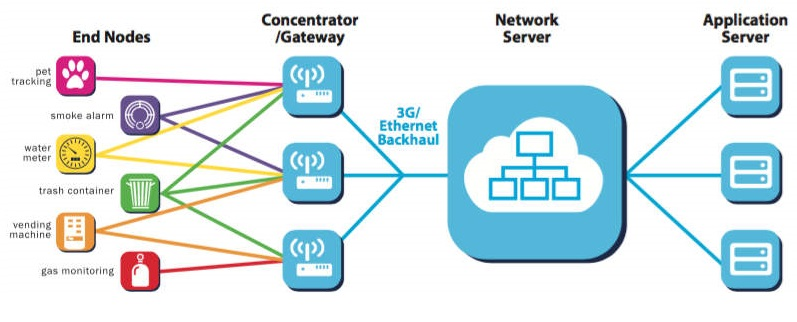
\includegraphics[width=.80\textwidth]{assets/lora-network-architecture.png} 
  \caption{Representação da relação entre os dispositivos LoRa (Adaptada de \cite{lora2021architecture}).}
  \label{fig:end-nodes-gateways} 
\end{figure}

% ----
\subsection{HTTP/HTTPS}
\label{fund:http}
Inicialmente utilizado pelo \textit{World-Wide Web}, WWW, em 1990, como o protocolo base da internet por ser uma protocolo leve e rápido para transições de informações em sistemas distribuídos, o \textit{Hypertext Transfer Protocol}, HTTP, é um protocolo que tramite documentos de diversos formatos através da sistemas distribuídos, mais conhecido pela sua disseminação pela internet \cite{berners1996hypertext}. Quanto anos depois, em 1994, a Netscape Communications criou o HTTPS, uma implementação do HTTP adicionando uma nova camada, a de segurança, utilizando-se do protocolo SSL/TLS, um protocolo que fornece segurança entre comunicações sobre rede de computadores.

O HTTP funcionando baseado no paradigma de cliente e servidor, onde o cliente estabelece uma conexão fazendo uma requisição solicitando algo ao servidor, e o servidor por sua vez, o responde enviando uma mensagem.  Tais requisições possuem um método atrelado a ele, esses métodos são usados semanticamente, com o objetivo de organizar e dividir suas responsabilidade, os métodos mais utilizados são: GET, POST, PUT e DELETE. o GET é usado quando o cliente solicita dados ao servidor, o POST quando o cliente quer enviar alguma nova informação, o PUIT é semelhante ao POST, entretanto é referente a atualização de um dados existente e o DELETE é um requisição pedindo a remoção de uma determinada informação \cite{mozilla2019http}.

Essas mensagens que transitam entre clientes e servidores, são compostas por linhas de textos dividas em três blocos como pode ser visto na figura \ref{fig:post-request}, o primeiro bloco consiste em uma linha com o método da requisição, a url, ou seja, o caminha do documento seguido pela a versão do protocolo; o segundo bloco são referentes ao cabeçalho HTTP, responsável por fornecer informações e metadados ao servidor, como o tipo de dado transitado ou dados que alteram seu comportamento; o terceiro bloco é respectivo ao bloco de dados, esse bloco é opcional dependendo do tipo de requisição realizada, mais utilizado pelos métodos POST e PUT.

\begin{figure}[H]
  \centering
  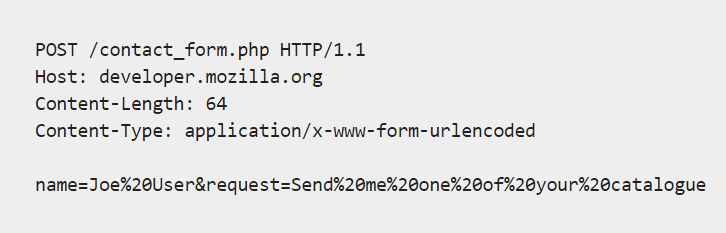
\includegraphics[width=.80\textwidth]{assets/post-request.png} 
  \caption{Exemplo de uma requisição POST (Retirado de \cite{mozilla2019http}).}
  \label{fig:post-request} 
\end{figure}

% ---
\section{Plataforma de prototipagem}
\label{fund:plataforma-proto}

% ---
\section{Sensor DHT-22}
\label{fund:dht-22}
O sensor DHT-22 é um sensor de temperatura e umidade da família de sensores DHT comumente utilizado em aplicações da IoT por ser um sensor pequeno(como podemos ver na figura \ref{fig:dht-22}) e possuir um baixo custo. Ele opera na faixa de 3.3 a 6 Volts e consegue capturar dados de temperatura entre -40°C a 80°C e umidade entre 0\% a 100\% RH, com uma acurácia de 0.5°C e 2\% RH, respectivamente \cite{datasheetDHT22}.

\begin{figure}[H]
  \centering
  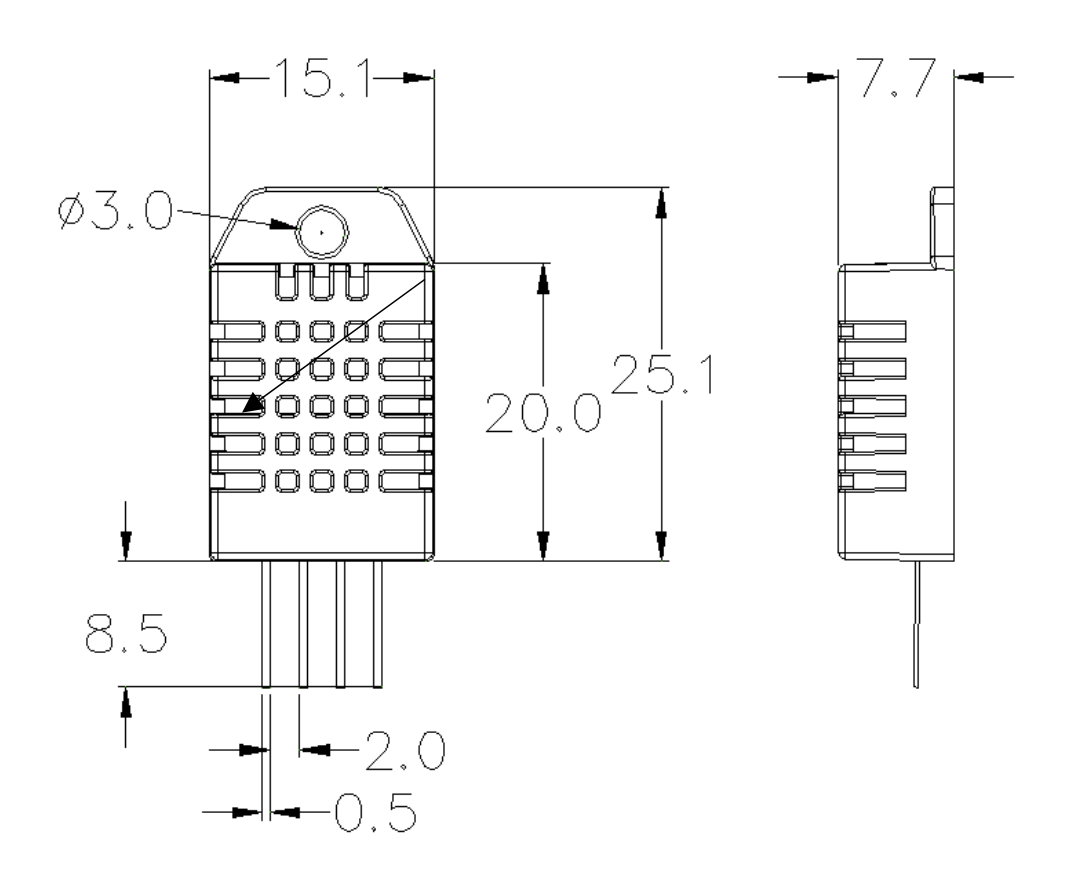
\includegraphics[width=.80\textwidth]{assets/dht-22.png} 
  \caption{Dimensões em milímetros do sensor DHT-22 (Retirado de \cite{datasheetDHT22}).}
  \label{fig:dht-22} 
\end{figure}

% ---
\section{Servidor}
\label{fund:servidor}
Um servidor é um sistema de computação centralizada, responsável por fornecer serviços em uma rede de computadores, tais serviços variam conforme a necessidade do sistema, podendo ser um controlador de domínio, provedor de arquivos, de impressão, de e-mails entre outros. No modelo cliente/servidor (figura \ref{fig:client-server-model}), por sua vez, o servidor é responsável por receber as requisições de clientes, provendo informações e dados de acordo com a demanda.

\begin{figure}[H]
  \centering
  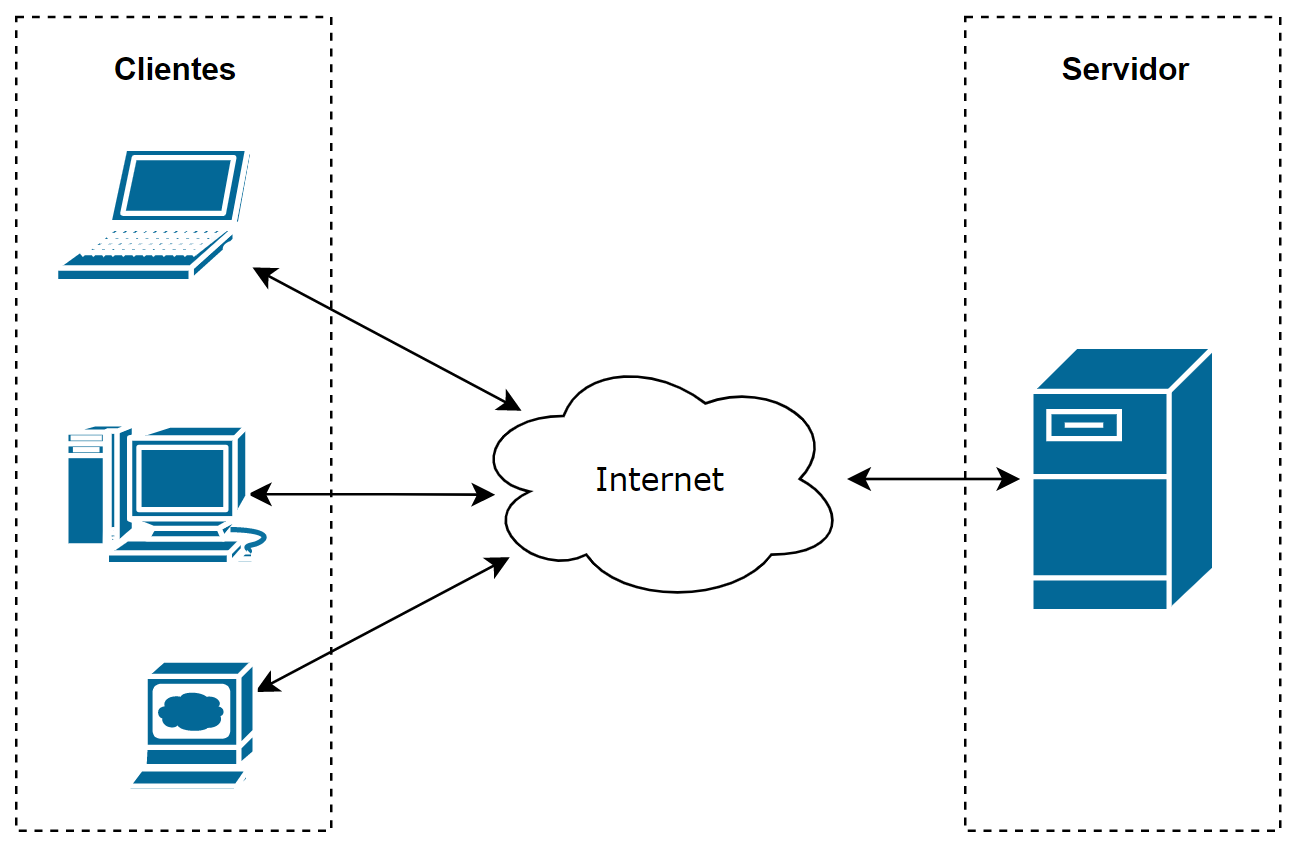
\includegraphics[width=.80\textwidth]{assets/client-server-model.png} 
  \caption{Representação do modelo cliente/servidor (Autoral).}
  \label{fig:client-server-model} 
\end{figure}

% ----
\subsection{Node.js}
\label{fund:node}
Em 2009, Ryan Dahl criou o Node.js ou simplesmente Node, um ambiente de código aberto de execução Javascript para ser utilizado por servidores (\textit{server-side}) baseado no interpretador V8 da Google. O objetivo do Node é fornecer uma forma de criar serviços com alta capacidade de escala, consumindo pouca memória e de fácil aprendizado. Apesar da linguagem de programação Javascript fornecer uma performance inferior as linguagens já existentes para esse objetivo, seu uso oferece dois grande beneficios, ser uma linguagem de fácil aprendizado e de grande uso por ser a linguagem padrão dos navegadores, e consequentemente do desenvolvimento web \cite{tilkov2010node}.

A forma de execução no Node é por eventos assíncronos, diferente da maioria dos outros ambientes modernos que utilizam threads do sistema operacional, SO. O Node usa apenas uma thread assíncrona principal que executa operações de entrada e saída de dados, E/S, chamada de \textit{Event Loop} \cite{nodejsAbout}. O \textit{Event Loop} funciona em um ciclo, escutando uma lista de chamas, onde são armazenadas as requisições recebidas, e as direcionando cada uma para uma Thread a parte, que executará a função recebida, como podemos ver na figura \ref{fig:event-loop-node}. A priori, o  Node possui quatro Threads trabalhadoras, responsáveis por executar as funções, entretanto é possível configurar dependendo da máquina onde está sendo efetuado a instância do Node.

\begin{figure}[H]
  \centering
  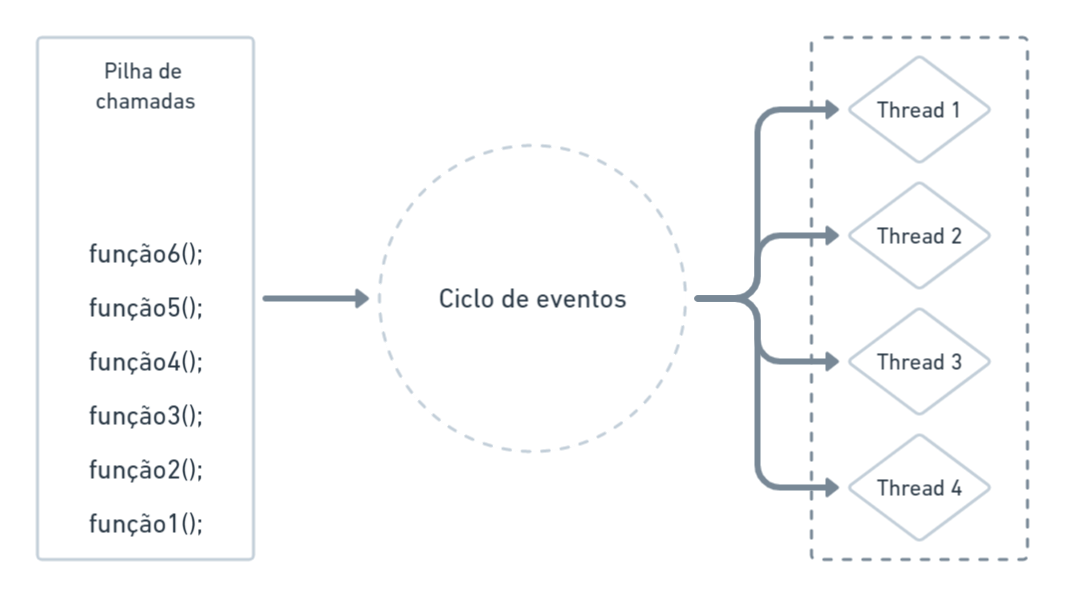
\includegraphics[width=.80\textwidth]{assets/event-loop-node.png} 
  \caption{Ciclo de eventos no Node (Autoral).}
  \label{fig:event-loop-node} 
\end{figure}

% ----
\subsection{InfluxDB}
\label{fund:influxdb}
O InfluxDB é um banco de dados que armazena series temporais (\textit{data series database}), ou seja, sua chave é o tempo e sua forma de armazenagem de dados é em ordem cronológica. Ele foi projetado para lidar com grandes cargas de escrita e consulta, perfeita para armazenar dados em tempo real, como monitoramento de DevOps, métricas de aplicativos, big data e dados de sensores da IoT \cite{giacobbe2018implementation}. De forma geral, séries temporais acabam se tornando gráficos em função do tempo em um determinado período, por exemplo a temperatura de um freezer ao decorrer do dia, podendo assim ver facilmente a máxima, a minima e suas variações. Esses dados podem ser também coletados e feito uma analise mais complexa usando qualquer ferramente estatística, dependendo da sua necessidade.

O InfluxDB é composto por \textit{databases} (bancos de dados), \textit{measurements} (medições), \textit{fields} (campos) e \textit{tags}. Podemos representar essa estrutura como conjuntos como podemos ver na figura \ref{fig:influxdb-struct}, no InfluxDB é possível ter inúmeros \textit{databases}, onde cada \textit{database} contém suas \textit{measurements} que são tabelas de dados correspondente a algum dado em específico, por exemplo, se tivermos 2 sensores que coletam dados diferentes, cada sensor viraria um \textit{measurement}, e cada \textit{measurement} é composto  de dois tipo de atributos, os \textit{fields}, onde ficam os dados da sua medida, e as \textit{tags}, que são campos de dados que diferem \textit{fields} por serem campos indexáveis, feitos exclusivamente para realizar buscas, por exemplo, é comum adicionar uma \textit{tag} que seja um identificador do dispositivo que coletou esse medida.

\begin{figure}[H]
  \centering
  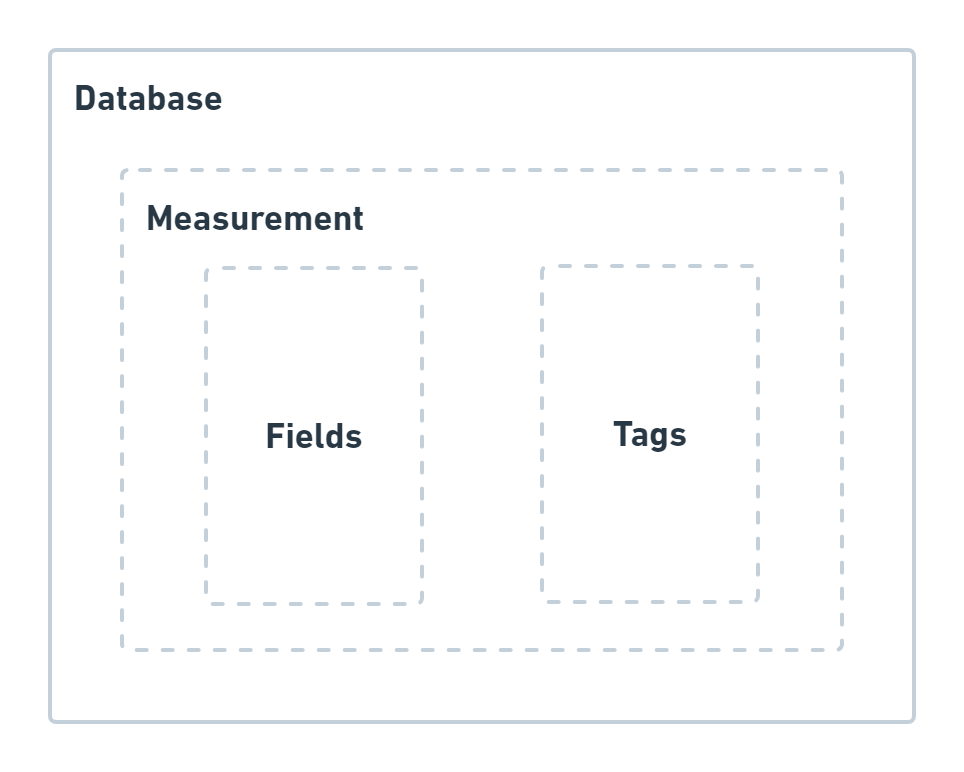
\includegraphics[width=.80\textwidth]{assets/influxdb-struct.png} 
  \caption{Composição de um banco de dados do InfluxDB (Autoral).}
  \label{fig:influxdb-struct} 
\end{figure}

% ----
\subsection{Docker}
\label{fund:docker}
Docker é uma plataforma \textit{open source}, desenvolvida utilizando a linguagem de programação GO pela Google com o objetivo de criar facilmente  ambientes isolados (containers) com um alto desempenho e que sejam portáteis, sendo uma opção em relação as virtualizações. Desta maneira, é possível, por exemplo, criar inúmeras aplicações usando as mesmas tecnologias, cada uma em um \textit{container} diferente e nenhuma vai interferir na outra, e todas na mesma máquina, e se for preciso replicar em outra máquina, é possível criar uma imagem do container e instalar o mesmo ambiente nesta outra máquina.

Em comparação com as virtualizações, os containers não precisam de um sistema operacional, apenas o essencial para executar determinada função. Dessa forma, os containers conseguem ter um controle maior, consomem menos recursos, ganham uma maior flexibilidade e uma manutenibilidade. Podemos ver a comparação entre virtualização e containers na figura abaixo.

\begin{figure}[H]
  \centering
  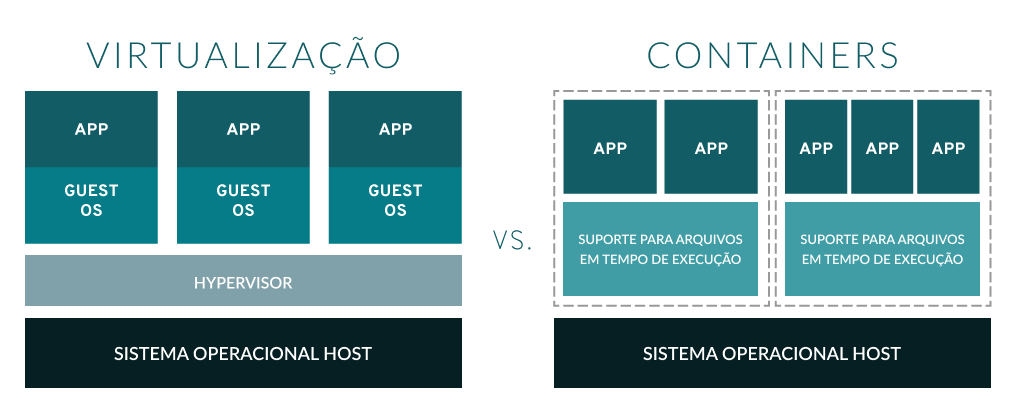
\includegraphics[width=.80\textwidth]{assets/virtualization-vs-containers.png} 
  \caption{Comparação entre o modelo de virtualização e modelo de containers (Adaptada de \cite{redhat2020Containers}).}
  \label{fig:virtualization-vs-containers}
\end{figure}

% Referencias
% - https://www.opservices.com.br/o-que-e-docker/
% - https://www.meupositivo.com.br/panoramapositivo/container-docker/
% - https://www.treinaweb.com.br/blog/no-final-das-contas-o-que-e-o-docker-e-como-ele-funciona/

% % ---
\section{Aplicativo móvel}
\label{fund:app}
Aplicativo móvel, APP, é um \textit{software} desenvolvido especificamente para dispositivos móveis, como telefones celulares, tablets, relógios inteligentes entre outros. Cada SO utiliza uma determinada linguagem de programação para desenvolvedores poderem criar os apps. Com uma grande diversidade de sistemas operacionais, com uma linguagem de programação distintas, transformam o desenvolvimento de aplicativos multiplataformas mais trabalhoso e repetitivo, pois tem que ser programada uma versão diferente para cada plataforma. Tendo esse problema em mente, várias formas de programação híbridas foram criadas, com o princípio de poder programar utilizando apenas uma código para várias plataformas distintas, dentre elas, as duas que mais se destacam atualmente são o Flutter e o React Native.

% ----
\subsection{React Native}
\label{fund:react-native}
O React Native é um \textit{framework} para desenvolvimento nativo voltado para dispositivos para os dois principais SO móveis atualmente, Android e iOS. Ele é de código aberto, mantido pelo Facebook e sua comunidade.  Ele é um \textit{framework} bastante popular, utilizado por grandes empresas globais atualmente, como Netflix, Uber, a própria Facebook e empresas brasileiras como o EBANX e a Globo \cite{empresasbrreact}.

O React Native utiliza a linguagem JavaScript como principal e a renderiza para código nativo, para isso é adicionado uma camada em JavaScript, chamada de \textit{Bridge} que se comunica com o sistema operacional, mandando comandos para renderizar os componentes nativos \cite{docreactnative}.

% ---
\section{Trabalhos Relacionados}
\label{fund:trabalhos-relacionados}